\documentclass[10pt,conference,compsocconf]{IEEEtran}

%\usepackage{times}
%\usepackage{balance}
\usepackage{url}
\usepackage{graphicx}
\usepackage{subcaption}
\usepackage{float}
\usepackage{amsmath, amssymb}
\usepackage{algorithmicx}
%\usepackage[ruled]{algorithm2e}
\usepackage[noend]{algpseudocode}

% bold paragraph titles
\newcommand{\mypar}[1]{{\bf #1.}}

\begin{document}
\title{In-painting with Savvy}

\author{
  Seijin Kobayashi, Frank Fu Lanke, Norman Juchler\\
  Department of Computer Science, ETH Zurich, Switzerland
}

\maketitle
\begin{abstract}
  A critical part of scientific discovery is the
  communication of research findings to peers or the general public.
  Mastery of the process of scientific communication improves the
  visibility and impact of research. While this guide is a necessary
  tool for learning how to write in a manner suitable for publication
  at a scientific venue, it is by no means sufficient, on its own, to
  make its reader an accomplished writer. We also describe the rules
  for submission in the computational intelligence laboratory.
  This guide should be a
  starting point for further development of writing skills.
\end{abstract}
\section{Introduction}
\label{sec:introduction}
Inpainting is an image processing technique used to infer the value of unknown pixels using the information apparent in the original image. One application for this method is image restoration where single pixels or larger scratches are missing, e.g. due to defective image acquisition or the age-driven deterioration of video footage. Another very common application is the removal of certain parts of an image, like watermarks or user-selected objects in the image. Figure \ref{fig:apps} shows examples for input images that can be treated by inpainting methods. Throughout this paper we assume that it is known beforehand which pixels have to be reconstructed. The extraction of defective regions in the image is not discussed here.

\begin{figure*}[t]
	\centering
	\begin{subfigure}{.5\columnwidth}
	   \centering
	   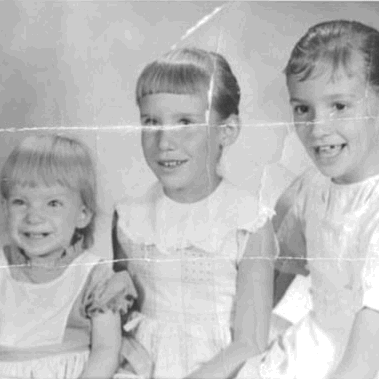
\includegraphics[width=.9\columnwidth]{graphics/3children_original_cropped.png}%
	      \caption{Image restoration
	      \label{fig:apps:image_restoration}
	   }
	\end{subfigure}\hfill%
	\begin{subfigure}{.5\columnwidth}
	   \centering
	   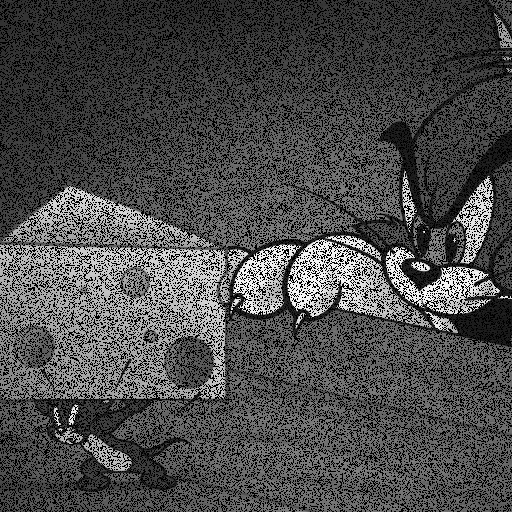
\includegraphics[width=.9\columnwidth]{graphics/TomAndJerry_512x512_pepper_in.png}%
	      \caption{Noise removal
	      \label{fig:apps:noise_removal}
	   }
	\end{subfigure}\hfill%
	\begin{subfigure}{.5\columnwidth}
	   \centering
	   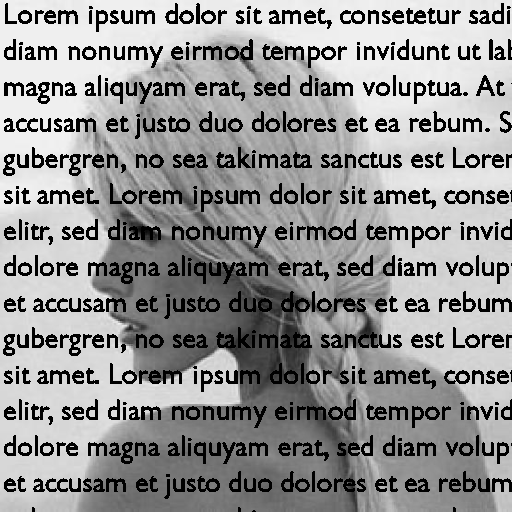
\includegraphics[width=.9\columnwidth]{graphics/claudia_512x512_mask_in.png}%
      	   \caption{Removal of watermarks
	      \label{fig:apps:watermarks}
	   }
	\end{subfigure}\hfill%
	\begin{subfigure}{.5\columnwidth}
	   \centering
	   
\includegraphics[width=.9\columnwidth]{graphics/object_removal_gray.png}%
      	   \caption{Object removal
	      \label{fig:apps:object_removal}
	   }
	\end{subfigure}\hfill%
	\caption{Sample applications for inpainting. (Images \ref{fig:apps:image_restoration}), \ref{fig:apps:noise_removal}), and \ref{fig:apps:watermarks}) are taken from \cite{CIL2015}, \ref{fig:apps:object_removal}) is from \cite{criminisi2004region})
	   \label{fig:apps}
	}
\end{figure*}

\mypar{Existing work}
Many different techniques exist for inpainting, see for example \cite{tauber2007review} for a review of methods originating in the domain of computer vision. A very common approach is referred to as \textit{texture-synthesis} where the objective is to remove (potentially large) objects from an image by mimicking the surrounding region of the to-be-removed objected. Very popular in the image processing community is the method described by Criminisi et al. \cite{criminisi2004region}, an onion-peel approach where local gradients steer the fill-in procedure, which helps to not only preserve texture but also structure.

Recently, inpainting driven by sparse encoding, a concept from the domain of statistical learning, became popular, see for example \cite{fadili2009inpainting} or \cite{elad2005simultaneous}. 

\mypar{Our approach}
The method presented here is based on sparse coding of image patches, which we combine with ideas that are inspired by the works of \cite{criminisi2004region}. The novelty of our patch-based method consists of the combination of the following components:
\begin{itemize}
   \item Valuable Information Propagation (VIP): Use evidence found in neighbouring patches for the sparse coding.
   \item Confidence Blending (CB): Redundant reconstruction of missing pixels by overlapping patches.
   \item A scheme to learn under-complete dictionaries that allow a reliable and fast encoding.
\end{itemize}

\mypar{Structure of the text} In section \ref{sec:methods} the proposed method is presented in depth. Section \ref{sec:results} presents our implementation which is then discussed in the subsequent section \ref{sec:discussion}. 
\section{Methods (The Structure of a Paper)}
\label{sec:methods}
\label{sec:structure-paper}



\subsection{Dictionary learning}

Another direction in which we investigated is the construction of the dictionary we would use for our sparse coding. The nature of a dictionary not only determines the quality of the inpainting result, but also the speed of the inpainting process, depending on the size of the dictionary as well as the degree of sparseness reachable with it. 
The choice of dictionary was particularly of interest in our case to improve the running time. The approach we adopted for the reconstruction of the image would a priori assure a good quality of the reconstruction, however on the expense of the time necessary for the reconstruction, hence the need of a dictionary which would limit this trade-off without affecting too much the improved quality of the reconstruction.
With this objective in mind, we built a under-complete dictionary on the space of patches of size 16x16, composed of 64 atoms (25 percent of the total dimension), by applying the approximate K-SVD algorithm on a training data customized for our need. We also paid particular attention to the initialization of the learning process, since this method is known to be initialization-sensitive [TODO REF]. In the rest of this section we will refer to the space of patches of size 16x16 as $E$.

\mypar{K-SVD algorithm}
The algorithm takes a training set of patches $X$, and learn a dictionary $U$, starting from an initialized value of $U$ and iteratively learning to fit to $X$ in a more efficient way. 
For all dictionaries, we used this algorithm with 15 iterations, using the same training data set.

\mypar{Training Data set}
The dictionary being under-complete, loss of information will inevitably occur. The atoms will hence need to be very efficient in reconstructing the image without losing important information. In other words, the atoms need to be able to describe characteristics of patches that have a high-variability among the kind of patches that we want to reconstruct. The aspects of patches with low-variability can be easily estimated by the mean, with a minimal loss of information. 
To achieve this, we first gathered patches of size 16x16 extracted from 36 pictures of size 512x512, consisting of photography of cities, nature and animals. We then applied principal component analysis (PCA) on these patches to deduce the most significant subspace of $E$ of dimension 64, i.e. the subspace of $E$ that include the highest variability of value among patches of real-world photography. We then projected the whole training set as well as our learning process onto that subspace. That way, we ensure that the learned 64 atoms stay in this a priori significant subspace, without getting lost into the less-meaningful directions of $E$, allowing them to efficiently reconstruct a patch.

\mypar{Initialization}
The algorithm we chose is sensitive to the choice of the initial candidate, it optimizes it locally and greedily until no progress is possible. We implemented 2 main different ways to initialize the learning process:
\begin{itemize}
   \item From a known dictionary: in this method, we initialize the dictionary on a known dictionary, such as a 64-atom DCT (Discrete Cosine Transform) dictionary, or the 64 significant vectors obtained by applying PCA to the training set.  
   \item k-means initialization: in this method, we initialize the dictionary based on the training data set. We first center and normalize the training data, after which we apply the K-means algorithm with K=64 based on the euclidean norm, and use the normalized 64 centroids as initializing atoms. To improve the robustness of the K-mean algorithm, we applied the algorithm 10 times and chose the result which had the smallest mean pairwise-distance with other clustering. 
\end{itemize}
A randomly-generated atom initialization have also been implemented to serve as a reference for studying the efficiency of other initialization methods. 

Lastly, to compare the efficiency of the overall dictionary performance, we set the baseline reference as the standard complete DCT dictionary.




TODO: Subsection ``Background" to introduce roughly the concepts of sparse coding.

TOOD: Present our method.

TODO: Present baseline method and Criminisi method. (My suggestion is to compare the results of our algorithm with the class winner. They probably will like this approach. We probably won't beat the performance of the Criminisi approach in general, but we might be better in some cases, furthermore we will be faster for sure...


\section{Results (Tips for Good Software)}
\label{sec:results}
\label{sec:tips-software}
TODO: implementation details

TODO: details about benchmarking. How did we compare results? Which data sets did we use.

TODO: idea: use existign datasets for inpainting. Maybe we can found some in the web.


There is a lot of literature (for example~\cite{hunt99pragmatic} and
\cite{spolsky04software}) on how to write software. It is not the
intention of this section to replace software engineering
courses. However, in the interests of reproducible
research~\cite{schwab00}, there are a few guidelines to make your
reader happy:
\begin{itemize}
\item Have a \texttt{README} file that (at least) describes what your
  software does, and which commands to run to obtain results. Also
  mention anything special that needs to be set up, such as
  toolboxes\footnote{For those who are
  particularly interested, other common structures can be found at
  \url{http://en.wikipedia.org/wiki/README} and
  \url{http://www.gnu.org/software/womb/gnits/}.}.
\item A list of authors and contributors can be included in a file
  called \texttt{AUTHORS}, acknowledging any help that you may have
  obtained. For small projects, this information is often also
  included in the \texttt{README}.
\item Use meaningful filenames, and not \texttt{temp1.m},
  \texttt{temp2.m}. The code should also unzip into a sub-directory.
\item Document your code. Each file should at least have a short
  description about its reason for existence. Non obvious steps in the
  code should be commented.
\item Describe how the results presented in your paper can potentially
  be reproduced.
\end{itemize}

\section{Discussion (Computational Intelligence Laboratory Requirements)}
\label{sec:discussion}
\label{sec:cil}

TODO: discuss the results. Why is our method worse/better than the other one etc.

TODO: outlook. What could be done in order to improve the method.


Your semester project is a group effort. It consists of four parts:
\begin{enumerate}
\item The programming assignments you solve during the semester.
\item Developing a novel solution for one of the assignments, e.g. by
  combining methods from previous programming assignments into a novel
  solution.
\item Comparing your novel solution to previous assignments.
\item Writing up your findings in a short scientific paper.
\end{enumerate}

\subsection{Developing a Novel Solution}

As your final programming assignment, you develop a novel solution to
one of the four application problems. You are free to exploit any idea
you have, provided it is not identical to any other group submission
or existing Matlab implementation of an algorithm on the
internet\footnote{\url{http://www.ethz.ch/students/semester/plagiarism_s_en.pdf}}.

Two examples for developing a novel solution:
\begin{itemize}
\item You implemented a collaborative filtering algorithm based on
  dimension reduction as part of an assignment. Now you apply
  dimension reduction to inpainting.
\item You implemented both a clustering and a sparse coding algorithm
  for image compression. Now you combine both techniques into a novel
  compression method.
\end{itemize}

\subsection{Comparison to Baselines}

You compare your novel algorithm to \emph{at least two baseline
  algorithms}. For the baselines, you can use the implementations you
developed as part of the programming assignments.


\subsection{Write Up}

The submission must be in PDF form, using the \LaTeX{} template
corresponding to the IEEE style of publication. Refer to
Section~\ref{sec:latex-primer} for more information about preparing
your document. The document should be a maximum of {\bf 4 pages}.

\subsection{\LaTeX{} Primer}
\label{sec:latex-primer}

\LaTeX{} is one of the most commonly used document preparation systems
for scientific journals and conferences. It is based on the idea
that authors should be able to focus on the content of what they are
writing without being distracted by its visual presentation.
The source of this file can be used as a starting point for how to use
the different commands in \LaTeX{}. We are using an IEEE style for
this course.

\subsubsection{Installation}

There are various different packages available for processing \LaTeX{}
documents.
On Windows, use the Mik\TeX{} package (\url{http://miktex.org/}), and
on OSX use MacTeX
(\url{http://www.tug.org/mactex/2009/}). Alternatively, on OSX, you
can install the \texttt{tetex} package via
Fink\footnote{\url{http://www.finkproject.org/}} or 
Macports\footnote{\url{http://www.macports.org/}}.

\subsubsection{Compiling \LaTeX{}}
Your directory should contain at least 4 files, in addition to image
files. Images should be in \texttt{.png}, \texttt{.jpg} or
\texttt{.pdf} format.
\begin{itemize}
\item IEEEtran.cls
\item IEEEtran.bst
\item groupXX-submission.tex
\item groupXX-literature.bib
\end{itemize}
Note that you should replace groupXX with your chosen group name.
Then, from the command line, type:
\begin{verbatim}
$ pdflatex groupXX-submission
$ bibtex groupXX-literature
$ pdflatex groupXX-submission
$ pdflatex groupXX-submission
\end{verbatim}
This should give you a PDF document \texttt{groupXX-submission.pdf}.

\subsubsection{Equations}

There are three types of equations available: inline equations, for
example $y=mx + c$, which appear in the text, unnumbered equations
$$y=mx + c,$$
which are presented on a line on its own, and numbered equations
\begin{equation}
  \label{eq:linear}
  y = mx + c
\end{equation}
which you can refer to at a later point (Equation~(\ref{eq:linear})).

\subsubsection{Tables and Figures}

Tables and figures are ``floating'' objects, which means that the text
can flow around it.
Note
that \texttt{figure*} and \texttt{table*} cause the corresponding
figure or table to span both columns.


\subsection{Grading}

There are two different types of grading criteria applied to your
project, with the corresponding weights shown in brackets.
\begin{description}
\item[Competitive] \ \\
  The following criteria is scored based on your rank
  in comparison with the rest of the class.
  \begin{itemize}
  \item time taken for computation (10\%)
  \item average rank for all other criteria relevant to the task, for
    example reconstruction error and sparsity (20\%)
  \end{itemize}
  The ranks will then be converted on a linear scale into a grade
  between 4 and 6.
\item[Non-competitive] \ \\
  The following criteria is scored based on an
  evaluation by the teaching assistants.
  \begin{itemize}
  \item quality of paper (30\%)
  \item quality of implementation (20\%)
  \item creativity of solution (20\%)
  \end{itemize}
\end{description}

\subsection{Submission System}

The deadline for submitting your project report is Friday, 22 June
2012.
You need to submit:
\begin{itemize}
\item PDF of paper.
\item Archive (\texttt{.tar.gz} or \texttt{.zip}) of software. Please
  do not forget to include author information in the source archive.
\end{itemize}

\textbf{Important:} Please check the submission instructions on the webpage 
as it is the most updated instructions. 


\section{Summary}
\label{sec:summary}

Summary
\begin{appendix}
\section*{Acknowledgements}
The author thanks Christian Sigg for his careful reading and helpful
suggestions.
\end{appendix}
%\section*{Seijin's Snippets}
Here goes Seijin's text.
%\section{Franks's Snippets}
Here goes Franks's text.

\subsection{Formulation as a sparse coding problem:}

In general the inpainting problem can be seen as a Maximum Likelihood Estimation (MLE) problem where the objective is to fill the missing pixels with most likely values, given the observed data. We represent the known values of the image through sparse enconding and during the process, infer pixel values at the locations of the unknown pixels, using the characteristics of the encoding basis. Popular bases include Discrete Cosine Transforms (DCT), Haar wavelets etc. which demonstrate favorable qualities for image encoding as they exhibit characteristics similar to generic image features. To achieve the sparse encoding we use the matching pursuit algorithm which serves to meet the following criterion
 		z* \ni \arg\max_{z} ||\mathbf{M}(\mathbf{x}-\mathbf{U}\mathbf{z}) ||_2
		s.t. ||z_0||  \leqslant K      (insert equation line 36 lecture 9).
Where \mathbf{M} is the masking matrix, \mathbf{x} is the observed pixels, \mathbf{U} is the dictionary matrix and \mathbf{z} are its sparse coefficients. 

Inpainting through sparse coding relies on infering unknown values based on the impact that the known pixels incur on the chosen basis. Therefore, for a given genre of images it is advantageous to utilize a custom dictionary which can easily encode the given genre's typical image characteristics. For example  in (Elad, Querre, Donoho), curvelets were demonstrated to be specifically efficient at encoding cartoon images. 

So far in the technique mentioned, the image is divided into individual patches on which the sparse encodings are found. This approach disregards the spatial distribution of the occlusions and is hence sensitive to images where certain patches contain little known information. In (Criminisi) a method is proposed which first ranks the divided patches with a confidence criterion that favors patches with more known pixel values. Then, dense information from the boundary patches of the masked regions are propagated throughout the occluded region. Inspired by this work, we pursue here, two ways of propagating valuable image information beyond the boundaries of one patch.

\subsection{Valuable Information Propagation (VIP)}
To tackle the issue of densely populated masks, one of our approaches was to infer information from the surrounding, better known neighbours. The patches are ranked by a confidence criterion, similar to the works of (Criminisi et al.) we employ here the proportion of known pixel values within a patch, as a quality measure. Propagating information from better to poorer patches is then done by performing inpainting on an imaginary patch which is the concatenation of the poor patch's boundaries and its corresponding better neighbour. Once this imaginary patch's pixels have been infered, parts of the poorer neighbour's boundary missing pixels are chosen at random, and updated. This step allows for the propagation of information from the better neighbouring patch, while also reserving some of the final reconstruction influence for the poorer patch itself. The proportion of the masked pixels updated during this step is controlled by a parameter \epsilon \in \left] 0,1 \right[, which controls the amount of information propagated from the neighbour. The boundary width i.e. the band of pixels that make up the boundary is also parameterized as a function of the patch size. This value determines the autonomy that a given poor pixel has over its final image reconstruction. The algorithm works as follows

   \usepackage{algorithmicx}
    \usepackage[ruled]{algorithm}
    \usepackage[noend]{algpseudocode}

\vspace{-0.2cm}%
\alglanguage{pseudocode}
\begin{algorithm}[h]
\small
\caption{Valuable Information Propagation}
\label{Algorithm:VIP}
\begin{algorithmic}[1]
\Create{$\mathbf{Descending patch quality order}$}{vector $Rank$}
  %%  \LineComment{\emph{Quick check if $x$ is in mCBF}}
    \For {$i = 1 \to length(Rank)$}
            %%\If {$mCBF.C_{f_i(x)\%N}$ == 0}
                %%\State \textbf{return}
            %%\EndIf
	SparseCoding of patch $i$
	update mask vector in  \mathbf{M} and image vector in  \mathbf{X} corresponding to patch i
	
	    \For {$j = 1 \to #Neighbours$}
		\If {$#Masked values_j}$ >= \mathbf{threshold}}
               	 \State {Perform information propagation from i to j}
			update mask and pixel values of j
	            \EndIf
	    \EndFor
    \EndFor
    
\Statex
\end{algorithmic}
  \vspace{-0.4cm}%
\end{algorithm}

\subsection {Discussion on Using a shorter dictionary}

As discussed in (lecture 9 slide 38, to be referenced), the recovery of a representation using matching pursuit is prone to the coherence amongst the dictionary's atoms. For a fixed dimensionality, the more atoms contained in the dictionary, the higher the chances of there being greater coherence, leading to poorer reconstructions. The brevity of our learned dictionary not only allows for the low error reconstructions compared to baseline techniques as depicted in fig(to put in comparison figure), but also, does so at a faster rate since the matching pursuit process searches through less atoms. Reconstruction speed is of great consideration especially when concerned with inpaiting on large data sets, videos etc.

%\section*{Norman's Snippets}
Here goes Norman's text.

\bibliographystyle{IEEEtran}
\bibliography{report}
\end{document}
